\chapter{DTU Space coating facility}
This chapter is written as a manual introduction for future students employees who wish to use the multilayer coating facility at DTU Space. Several of the sections, such as those describing the development of the control software are not necessary for anything but to give a background on the considerations taken in the process.

\section{Overview}
The multilayer coating facility is the vacuum chamber placed in the laboratory that is otherwise known as the Multilab. It started out as a vapor deposition chamber for the SODART mission. Capable of vaporising a gold wire with a W rod in the center of the chamber, it would deposit a layer of gold on any mirror facing the center. The chamber was later upgraded with magnetrons, each with independent shutters.

The currently used magnetrons are attached to powerful DC power supplies that can deposit films atom-by-atom instead of the larger gold particles that would come from vaporisation. The upgrade made it possible to coat multilayers with d-spacings thinner than 3 nm and eventually became the coating method used for the NuSTAR mission.

The entire lab was moved from Rockefeller Institute near Rigshospitalet in Copenhagen during the summer of 2012. It was up running again around the summer of 2013 in the newly constructed building 328, the new home for DTU Space on DTU campus. In the new location, the lab is 50\% larger, has a double airlock (earlier just a single airlock), laminar airflow from ceiling mounted HEPA filters and various other improvements. The result is a considerably cleaner facility, which is important to avoid contaminants on optical substrates.

\section{Laboratory setup}
%In this section, the various instruments facilities will be described. Any reader not interested in using the Multilab can skip to section \ref{sec:ml_chamber}.
The vacuum chamber is the dominant piece of the laboratory, most of the computers, electronics and cooling in the lab is in some way connected to the chamber. Apart from the chamber, the lab consists of a downflow module, two fume hoods, a profilometer, a large clean room oven and various tables cupboards. Next to the lab is the Multilab Auxilliary Room, which houses the cooling heat exchangers and pumps, the rotary vane roughing pump, DC power supplies, and a large part of the extra storage needed for the lab. Additionally, there is a room in the basement that houses a ceramic oven that has a built in vacuum chamber, the room also serves to store hundreds of spare pieces of NuSTAR optic glass.

\subsection{Downflow module}
The downflow module is where the

\subsection{Fume hoods}

\subsection{Oven}

\subsection{Multilab auxilliary room}

\subsection{Multilab basement storage}

\subsection{Profilometer}

\section{Multilayer coating chamber}\label{sec:ml_chamber}

\subsection{Chamber, pumps \& valves}
Bell\\
Viton ring\\
Heaters\\
Roughing pump\\
Turbo pump

\subsection{Cathodes}
Powersupplies\\
Masks\\

\subsection{Gas flow controllers}

\subsection{Pressure gauges}
Baratron\\

\subsection{Rotating ring}

\subsection{Cathode shutters}

\section{Multilab control software}\label{sec:ml_software}

\subsection{The original control software}

\subsection{Considerations on the new software solution}
\begin{verbcode}
  SPEC> mra
\end{verbcode}

\section{Coating calibration}
To deposit a coating with the correct film layer thicknesses on a substrate, a calibration of the material combination is required. Four samples of 10 bilayer films are coated using the two materials. Each sample is placed on a separate mounting plate and each coated with a different thickness of both light and heavy materials. The samples are then measured using XRR and compared to an IMD model fit to get bilayer thickness (d-spacing) and thin/heavy material fraction ($\Gamma$) as seen in figure \ref{fig:irb4c-fit}.

\begin{figure}[!h]
  \center
  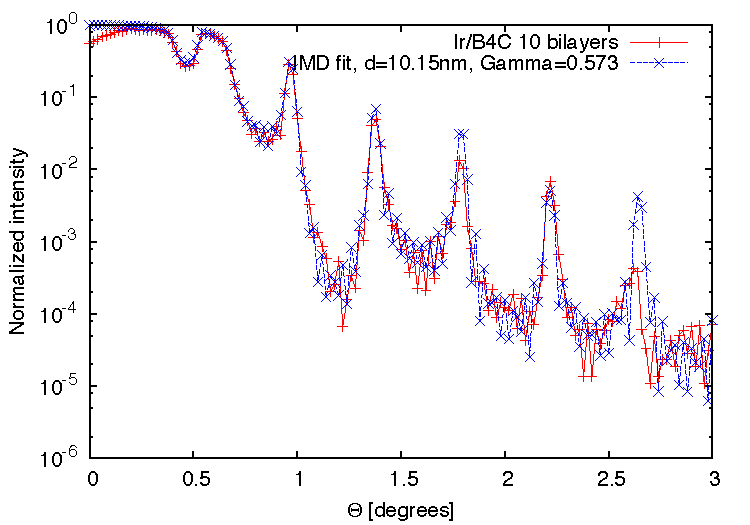
\includegraphics[height=6cm]{figures/chamber/si5811-fit.pdf}
\caption{\footnotesize XRR measurement of a 10 bilayer Ir/B$_4$C coating to calibrate for SPO coating. The measurement is fitted with an IMD model to determine d-spacing $\Gamma$.}\label{fig:irb4c-fit}
\end{figure}

The result for each sample is used to get the specific thickness of a material when coating with a given speed. Each result from the IMD model fitting is put into a table like the following:

%\begin{table}[!h]
\begin{center}
\begin{tabular}{c|c|c|c|c}
Sample & speed (Ir) & speed (B$_4$C) & d-Ir [nm] & d-B$_4$C [nm] \\
\hline
si5809 & 2623 & 473 & 2.42 & 2.54 \\
si5810 & 1445 & 338 & 3.21 & 3.88 \\
si5811 & 1011 & 236 & 4.33 & 5.81 \\
si5812 &  674 & 158 & 6.40 & 8.85 \\
si5813 & 281 & 225 & 14.55 & 7.49
\end{tabular}
\end{center}
%\caption{\footnotesize Calibration samples coated with 10 bilayer Ir/B$_4$C multilayers of different thickness. Each sample is measured using XRR and fitted to an IMD model. \label{tab:AFMsamples}}
%\end{table}

The d-spacings for a given material are plotted as a function of the inverse speed of the sample ring (v$^{-1}$) and fitted with a linear regression as seen in figure \ref{fig:calib-fit}. The $a$ and $b$ values of the linear regression are used directly to determine the speed of the sample ring to coat e.g. B$_4$C with a thickness of $d_{\mathrm{B}_4\mathrm{C}}$ like so:

\begin{eqnarray}
	v_{\mathrm{B}_4\mathrm{C}} = \frac{a}{d_{\mathrm{B}_4\mathrm{C}}-b}.
\end{eqnarray}

\begin{figure}[!h]
	\center
	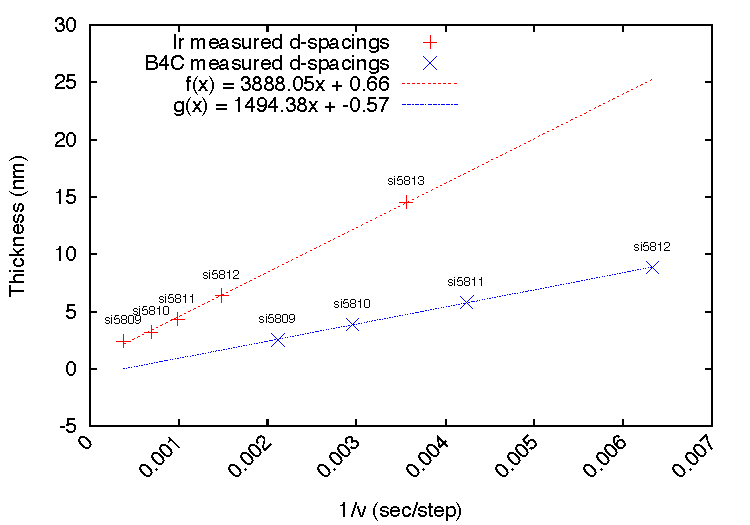
\includegraphics[height=4cm]{figures/chamber/calibration_plot-ir-b4c.pdf}
	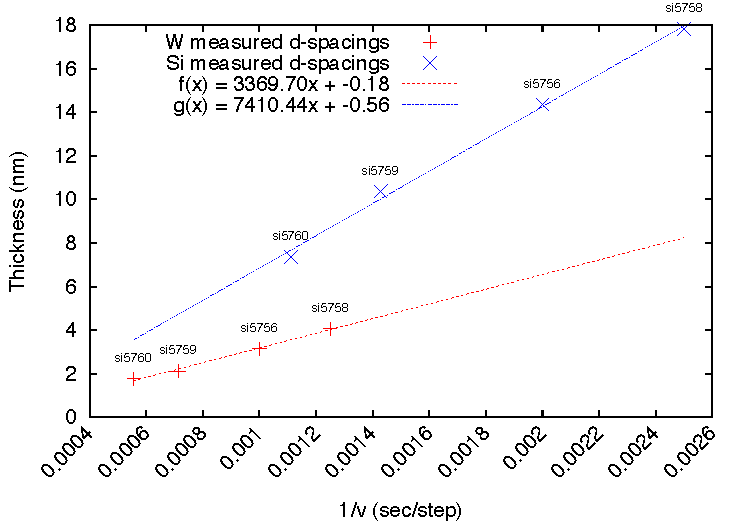
\includegraphics[height=4cm]{figures/chamber/calibration_plot-w-si.pdf}
\caption{\footnotesize Linear regression fits of calibration samples for Ir/B$_4$C (left) W/Si (right). Each datapoint is the XRR measured material thickness of one sample.}\label{fig:calib-fit}
\end{figure}
